\chapter{混合与溶解}\label{ch:g2:mixing-and-dissolving}

一块方糖落入一杯热茶中。勺子搅动，方糖碎裂，
片刻之后，已看不见任何东西：茶水的样子
与之前完全一样。然而，茶水现在尝起来是甜的。糖并没有
消失，它藏在茶水里。本章讨论的是把东西放在一起，
以及我们这样做时那些看似消失的东西。

\begin{omfigure}
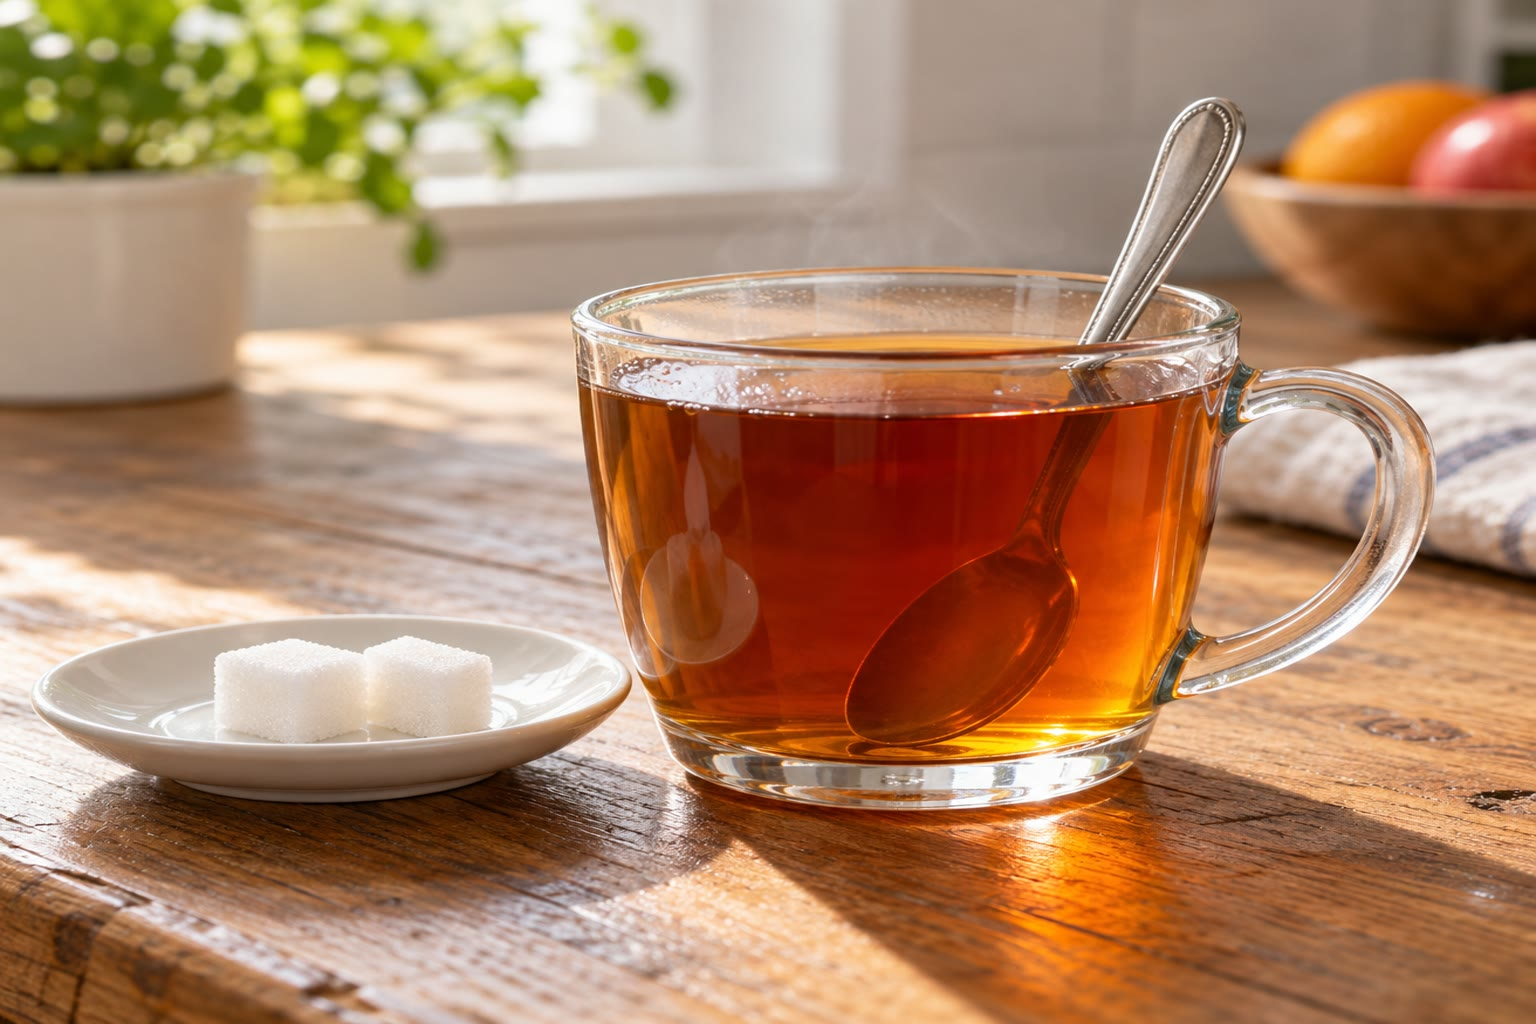
\includegraphics[width=0.55\linewidth]{images/book1/ai/g2-tea-sugar.jpg}

{\small 一杯茶和两块方糖。搅拌后，糖从视线中
消失了，但仍能从味道中尝出来。}
\end{omfigure}

\section{把东西混合在一起}

\begin{definition}[混合]\label{def:g2:mixing-and-dissolving:mix}
\emph{混合}\index{混合}是指把不同的东西放在一起，并且常常
加以搅拌。所得到的便是这些东西的混合物。
\end{definition}

\begin{example}[一碗麦片]\label{ex:g2:mixing-and-dissolving:muesli}
燕麦片、葡萄干、坚果和种子倒入同一个碗中：这就是混合物。
仔细看，每一种配料仍然看得见，
还能用手一一挑出来——葡萄干仍是葡萄干，坚果仍是坚果。
\end{example}

\begin{example}[糖浆与水]\label{ex:g2:mixing-and-dissolving:syrup}
两种液体也可以混合。把红色糖浆倒入一杯水中，
糖浆会以一缕缕颜色下沉；搅拌后，整杯水均匀地变成粉红色。
糖浆与水用肉眼已无法分辨。
\end{example}

\begin{omfigure}
\begin{minipage}[t]{0.48\linewidth}\centering
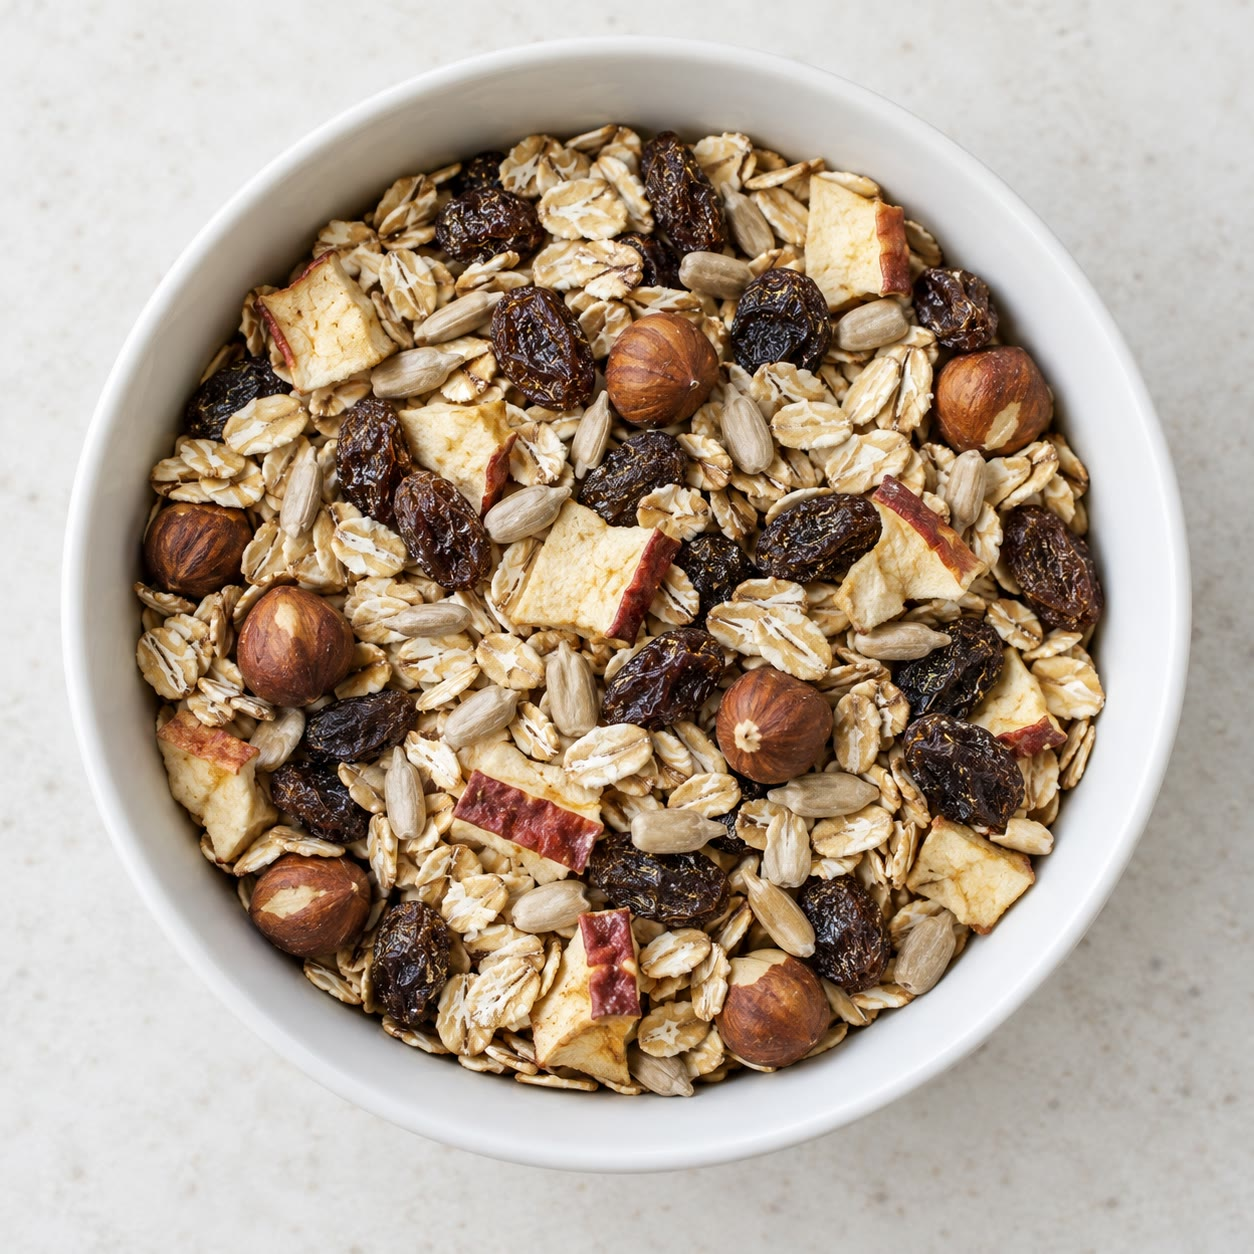
\includegraphics[width=\linewidth,height=4.6cm,keepaspectratio]{images/book1/ai/g2-muesli.jpg}

{\small 麦片：一种混合物，每一部分仍然都能看见。}
\end{minipage}\hfill
\begin{minipage}[t]{0.48\linewidth}\centering
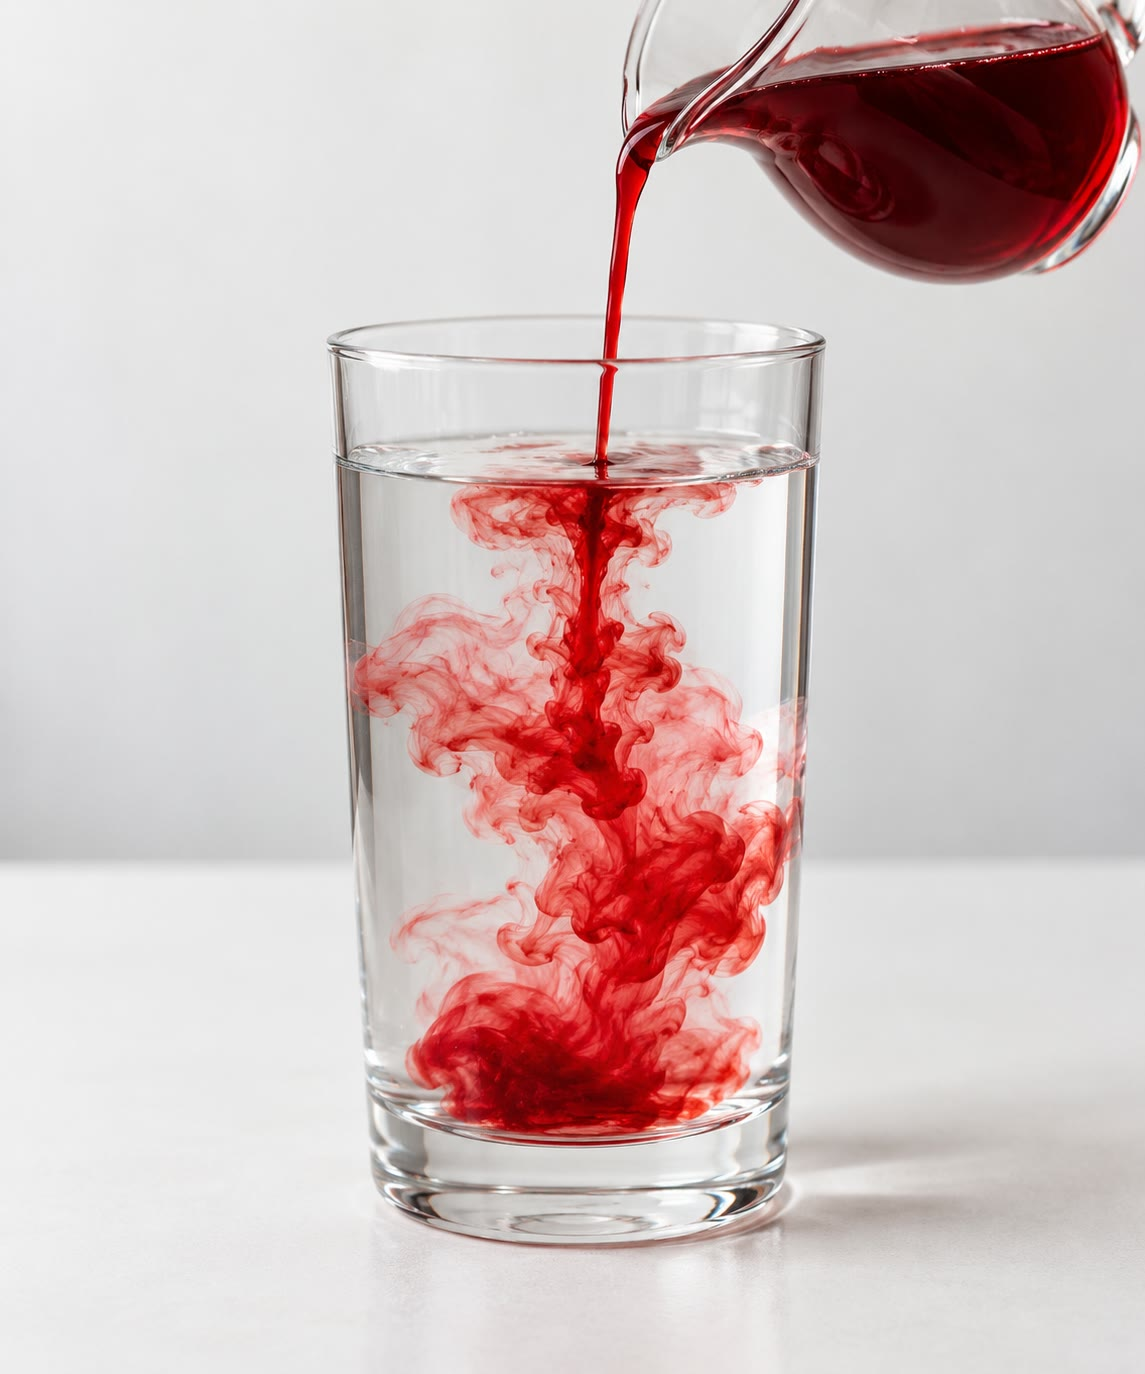
\includegraphics[width=\linewidth,height=4.6cm,keepaspectratio]{images/book1/ai/g2-syrup-in-water.jpg}

{\small 糖浆倒入水中：两种液体正在混合。}
\end{minipage}
\end{omfigure}

\begin{remark}[混合不会使物质消失]\label{rem:g2:mixing-and-dissolving:nothing-lost}
东西混合在一起时，既没有东西损失，也没有生成新物质。
燕麦片、葡萄干和坚果都还在碗里。
后面的章节会介绍如何把混合物重新分开。
\end{remark}

\section{能溶解的物质}

\begin{definition}[溶解与溶液]\label{def:g2:mixing-and-dissolving:dissolve}
固体放入水中并搅拌后，若从视线中消失，则称该固体在水中\emph{溶解}\index{溶解}，
并使液体变得
\emph{澄清}，即透明。食糖和食盐都能溶解。
所得的这种液体称为
\emph{溶液}\index{溶液}：糖水是糖的溶液，
咸水是食盐的溶液。
\end{definition}

\begin{example}[一杯水中的方糖]\label{ex:g2:mixing-and-dissolving:cube}
把一块方糖放在一杯静水的杯底。它的
棱角变软，体积变小，并有一缕缕波纹状的痕迹从它身上
穿过水体向上升起。若搅拌，一分钟之内就会消失；若不搅拌，
它仍会消失，只是慢得多。
\end{example}

\begin{remark}[澄清不等于无色]\label{rem:g2:mixing-and-dissolving:clear}
茶水是褐色的，糖浆水是粉红色的，但透过它们都能看到另一侧：
它们都是澄清的。溶液可以有颜色，但溶液中
绝不会有漂浮的小颗粒，也不会在底部有一层东西。
\end{remark}

\begin{method}[它能溶解吗？]\label{met:g2:mixing-and-dissolving:test}
要判断某种固体能否溶解在水中，可按下列步骤操作：
\begin{enumerate}
  \item 取少量该固体放入一杯水中；
  \item 搅拌，然后等待几分钟；
  \item 透过杯子观察：
    \begin{itemize}
      \item 澄清，且底部没有东西：该固体已溶解；
      \item 浑浊，或底部有一层东西：该固体未溶解。
    \end{itemize}
\end{enumerate}
\end{method}

\section{不能溶解的物质}

\begin{proposition}[沙子和粉笔不能溶解]\label{prop:g2:mixing-and-dissolving:not}
许多固体不能溶解在水中：沙子、粉笔、土壤、小石子、
面粉。放入水中搅拌，水会变浑浊；静置后，它们会下沉
并沉到底部，上层的水又变得澄清。
无论搅拌多久，它们都不会消失。
\end{proposition}

\begin{example}[一罐浑浊的水]\label{ex:g2:mixing-and-dissolving:mud}
把园子里的土壤放入一罐水中摇晃，水就变成褐色且浑浊。过了
一小时，泥土和小石子在底部形成一层深色沉积物，
几片枯叶漂浮在水面上，中间的水只是
有点浑浊。泥土并没有溶解。
\end{example}

\begin{omfigure}
\begin{minipage}[t]{0.48\linewidth}\centering
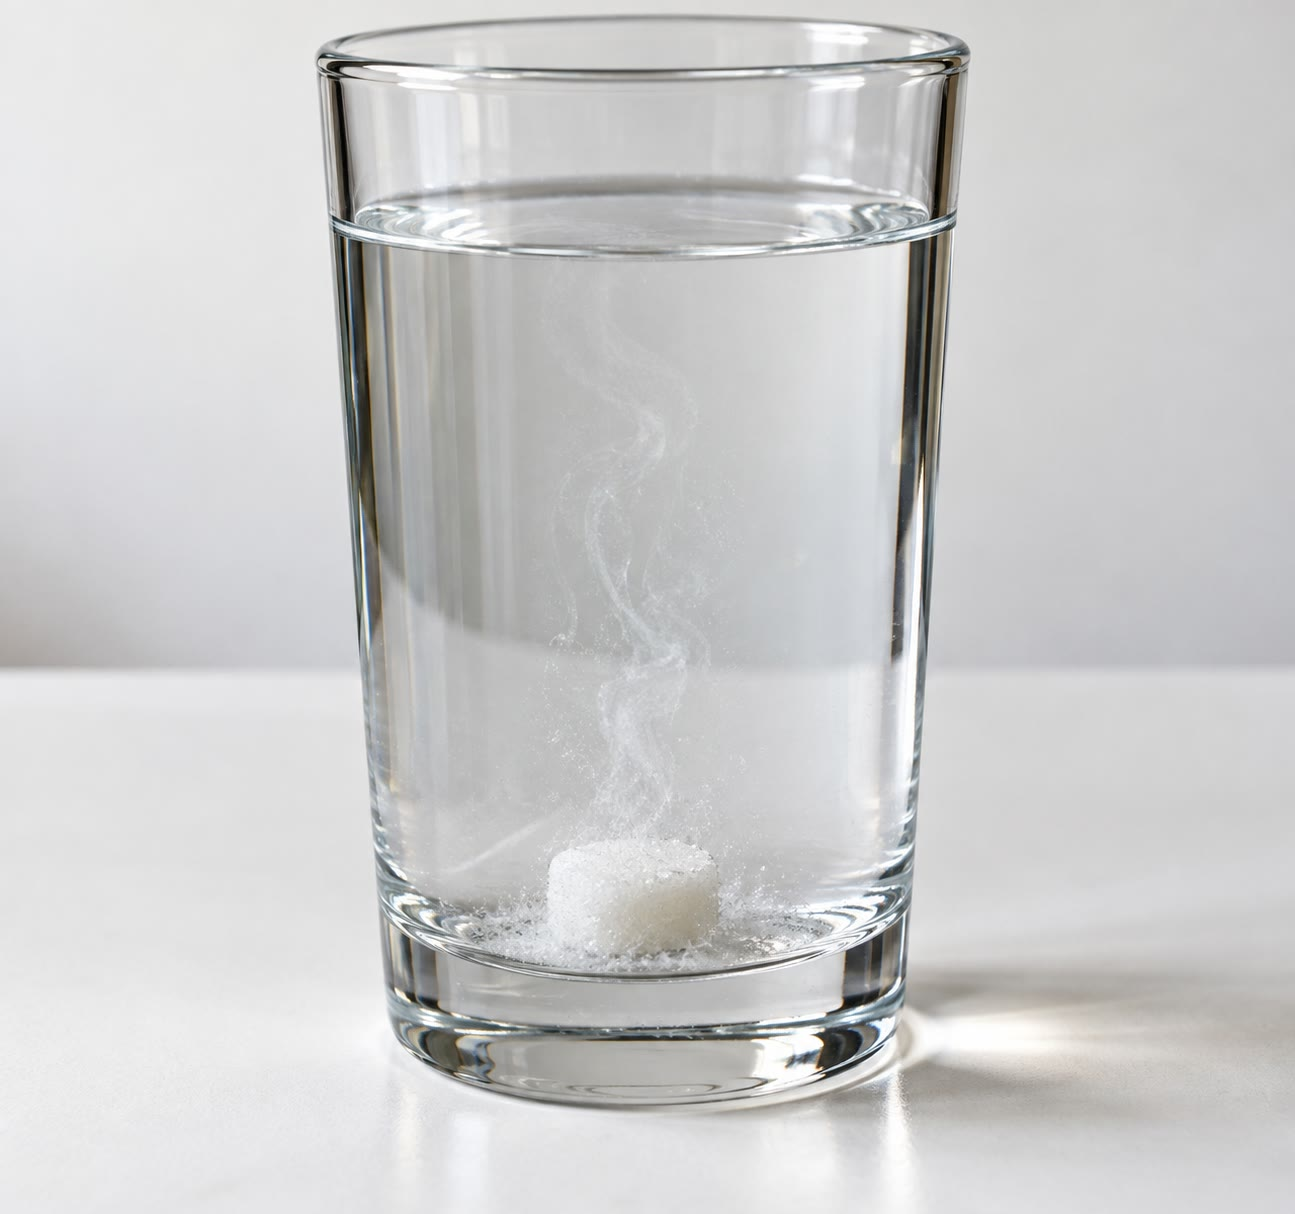
\includegraphics[width=\linewidth,height=4.6cm,keepaspectratio]{images/book1/ai/g2-sugar-cube-dissolving.jpg}

{\small 糖在溶解：条纹从方糖上升。}
\end{minipage}\hfill
\begin{minipage}[t]{0.48\linewidth}\centering
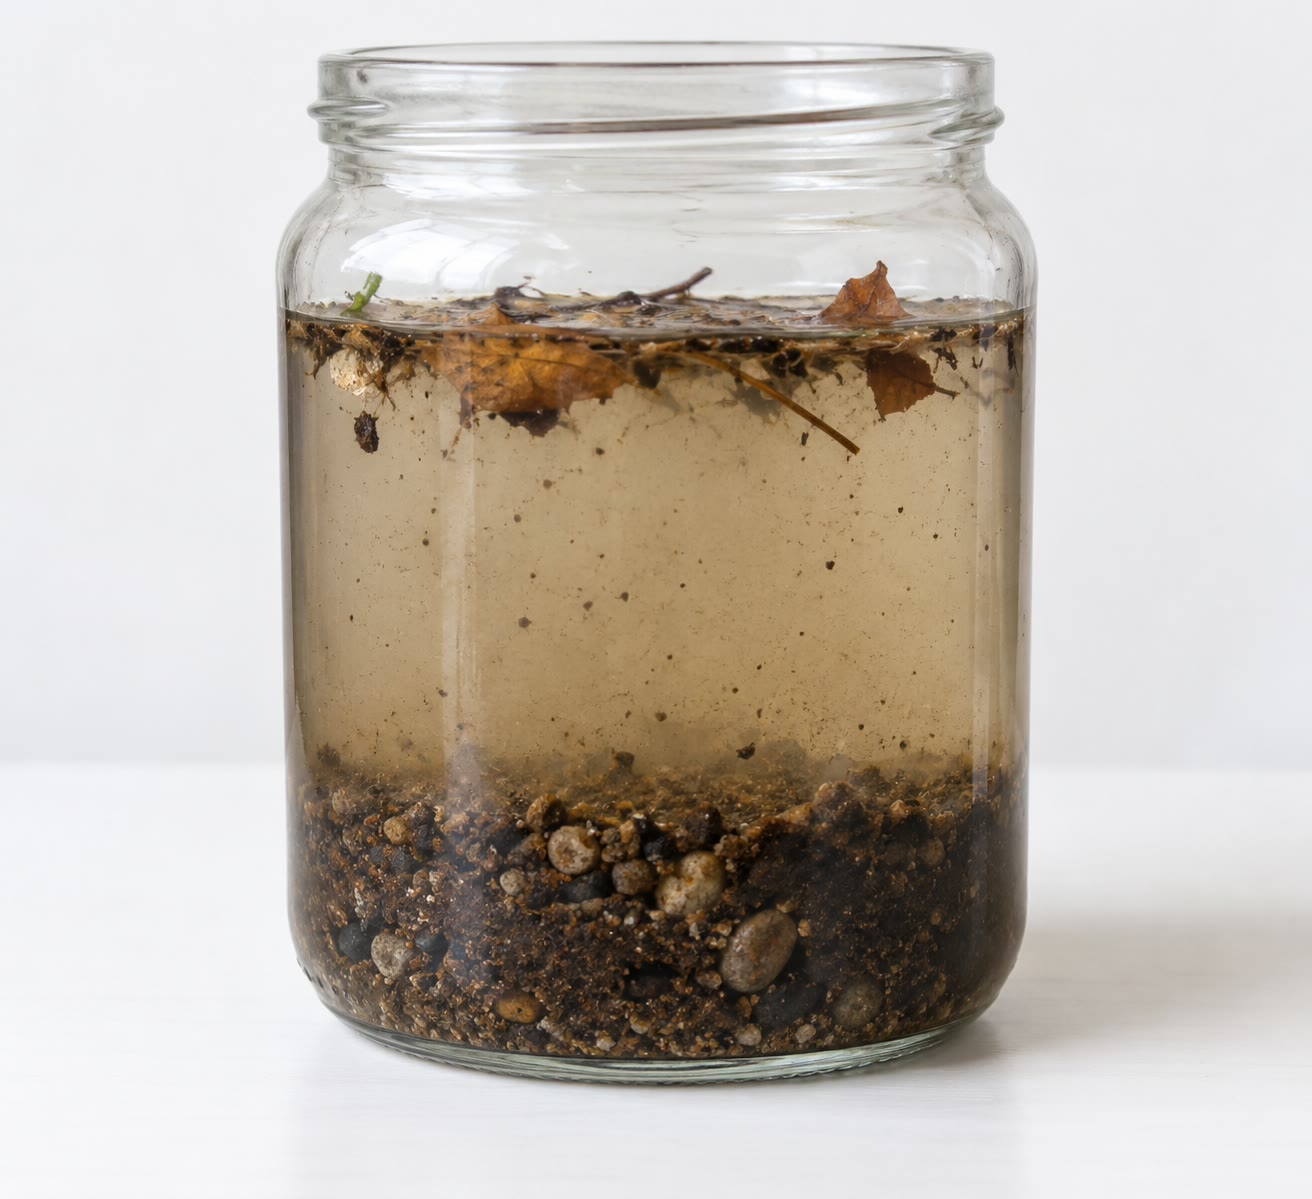
\includegraphics[width=\linewidth,height=4.6cm,keepaspectratio]{images/book1/ai/g2-muddy-jar.jpg}

{\small 泥土不溶解：它沉在底部。}
\end{minipage}
\end{omfigure}

\begin{omfigure}
\begin{tikzpicture}[font=\small, scale=1.35]
  \pic[transform shape] at (0,0) {beaker={0.7}{omWater!70}};
  \fill[brown!55] (4.2,0) rectangle (5.8,0.22);
  \pic[transform shape] at (5,0) {beaker={0.7}{brown!12}};
  \fill[brown!55] (4.2,0) rectangle (5.8,0.22);
  \draw[omGlass, line width=0.7pt] (4.2,0.22) -- (4.2,0) -- (5.8,0) -- (5.8,0.22);
  \foreach \x/\y in {4.4/0.32,4.75/0.45,5.1/0.3,5.5/0.5,4.6/0.7,5.3/0.8,4.9/1.0}
    \fill[brown!60] (\x,\y) circle (0.025);
  \node[align=center, anchor=north] at (0,-0.15)
    {\textbf{糖}放入水中搅拌：\\ 澄清，底部什么也没有};
  \node[align=center, anchor=north] at (5,-0.15)
    {\textbf{沙子}放入水中搅拌：\\ 浑浊，底部有一层};
  \draw[<-, omProp, thick] (6.0,0.11) -- (7.0,0.11)
    node[right, text=black] {沙子};
\end{tikzpicture}

{\small \cref{met:g2:mixing-and-dissolving:test}的检验：糖
溶解，沙子不溶解。}
\end{omfigure}

\section{溶解的物质仍在水中}

\begin{proposition}[溶解的固体仍在水中]\label{prop:g2:mixing-and-dissolving:still-there}
固体溶解时并没有消失，而是散布在
整杯水中，碎粒小得肉眼看不见。有两条线索说明它仍在
水中：
\begin{itemize}
  \item 甜茶尝起来是甜的，海水尝起来是咸的；
  \item 水干了以后，固体会留下来。
\end{itemize}
\end{proposition}

\begin{remark}[实验室里不尝味道]\label{rem:g2:mixing-and-dissolving:no-tasting}
茶是甜的，是因为茶是食物。在实验室里，没有人
会尝任何东西，哪怕是看起来像水的液体：
第二条线索，让水蒸干，才是化学家所用的方法。
\end{remark}

\begin{example}[来自海水的盐]\label{ex:g2:mixing-and-dissolving:salt-pans}
在一些阳光充足的海岸，海水被引入宽而浅的池塘。日复
一日，阳光把水晒干。留在池底的
白色盐粒被耙成一堆一堆，正是溶解在
海水中的盐。餐桌上的盐常常来自这样的池塘。
\end{example}

\begin{omfigure}
\begin{tikzpicture}[font=\small, scale=1.25]
  % day 1: a saucer of salty water
  \fill[omWater!80] (0,0.18) ellipse (1.25 and 0.22);
  \draw[omGlass, line width=0.7pt] (-1.5,0.3) .. controls (-1.2,-0.15) and (1.2,-0.15) .. (1.5,0.3);
  \draw[omGlass, line width=0.5pt] (0,0.3) ellipse (1.5 and 0.28);
  \node[align=center, anchor=north] at (0,-0.35) {一碟 \\ 咸水};
  % the sun
  \fill[ocYellow] (3.4,1.45) circle (0.28);
  \foreach \a in {0,45,...,315}
    \draw[ocYellow!90!orange, thick] ($(3.4,1.45)+(\a:0.36)$) -- ($(3.4,1.45)+(\a:0.52)$);
  \draw[->, thick, omProp] (2.0,0.3) -- (4.8,0.3)
    node[midway, below, text=black, align=center] {几个晴天 \\ 之后};
  % later: a white crust
  \begin{scope}[xshift=6.3cm]
    \draw[omGlass, line width=0.7pt] (-1.5,0.3) .. controls (-1.2,-0.15) and (1.2,-0.15) .. (1.5,0.3);
    \draw[omGlass, line width=0.5pt] (0,0.3) ellipse (1.5 and 0.28);
    \foreach \x/\y in {-0.9/0.12,-0.6/0.2,-0.3/0.08,0/0.18,0.3/0.1,0.6/0.2,0.9/0.12,
                       -0.45/0.28,0.15/0.27,0.75/0.3,-0.75/0.31}
      \fill[white, draw=black!45, line width=0.2pt] (\x,\y) rectangle ++(0.11,0.07);
    \node[align=center, anchor=north] at (0,-0.35) {水已蒸干：\\ 白色盐};
  \end{scope}
\end{tikzpicture}

{\small 水干了，溶解在其中的盐
留了下来。}
\end{omfigure}

\begin{omfigure}
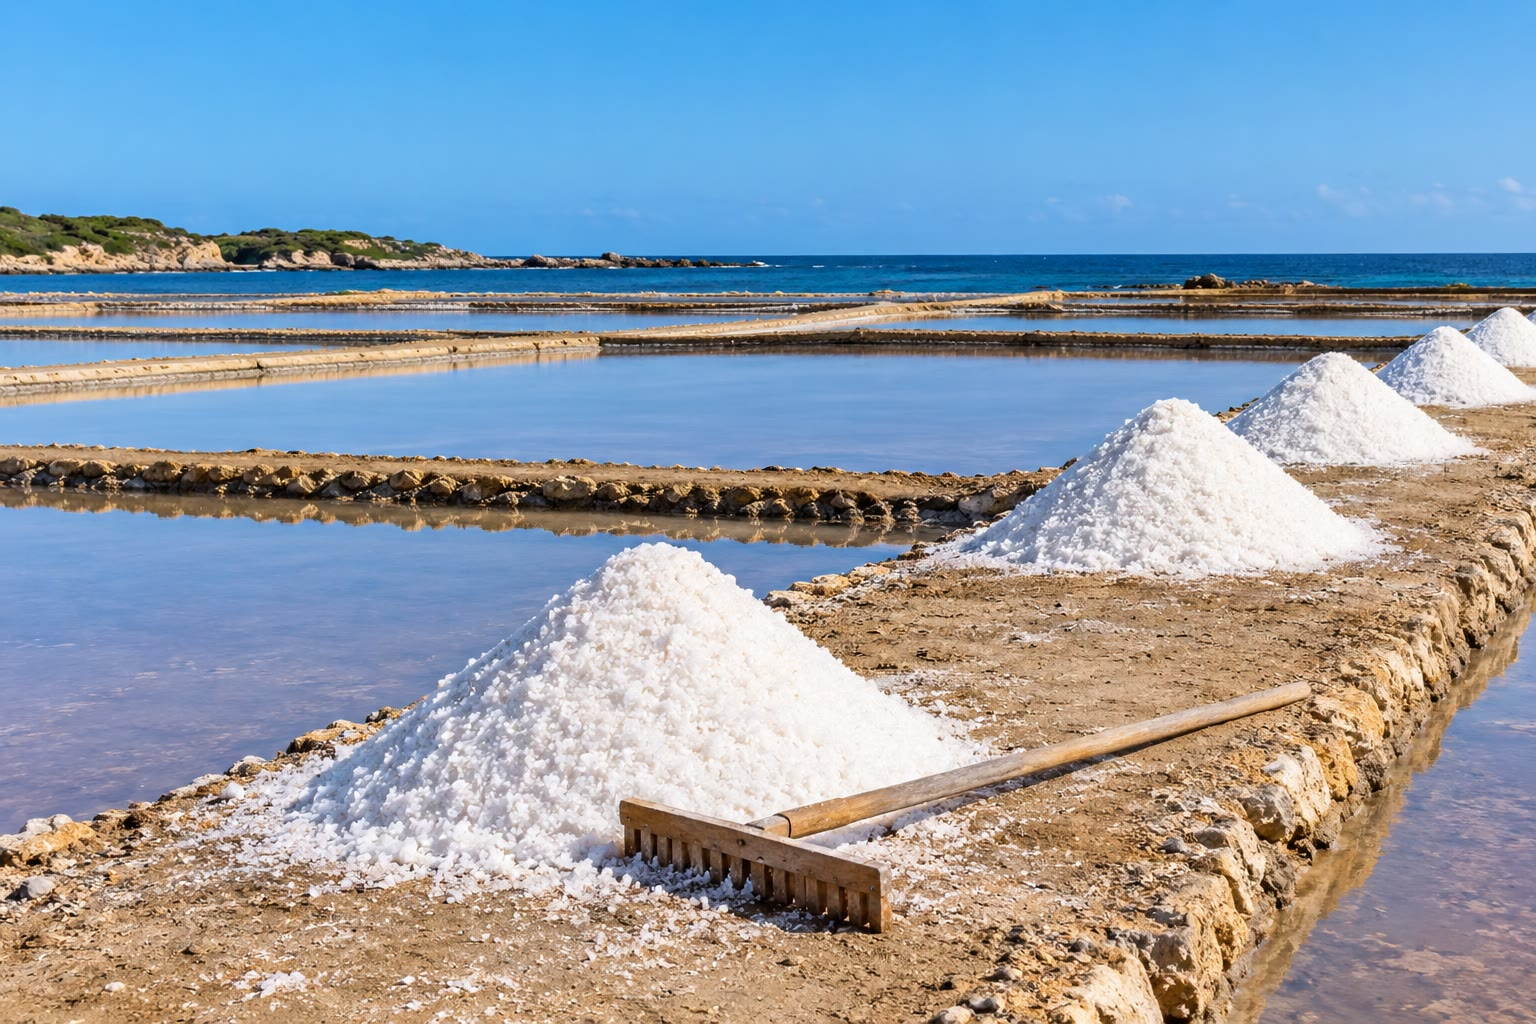
\includegraphics[width=0.62\linewidth]{images/book1/ai/g2-salt-pans.jpg}

{\small 海边的盐池：阳光晒干海水，盐
留成一堆堆白色的盐。}
\end{omfigure}

\begin{remark}[溶解不是熔化]\label{rem:g2:mixing-and-dissolving:not-melting}
人们常说糖在茶里“熔化”。其实不是：熔化是
冰块在阳光下自己变成液体的过程，
不需要水。糖在茶里则需要水，而糖
仍在水中，只是散开了。正确的说法是\emph{溶解}。
\end{remark}

\section{练习}

\begin{exercise}[$\star$]\label{exo:g2:mixing-and-dissolving:1}
下列哪些固体能溶解在水中，哪些不能？糖、
沙子、盐、粉笔、鹅卵石。
\end{exercise}

\begin{exercise}[$\star$]\label{exo:g2:mixing-and-dissolving:2}
什么是溶液？请举出本章中的两个例子。
\end{exercise}

\begin{exercise}[$\star$]\label{exo:g2:mixing-and-dissolving:3}
一碗麦片算不算一种混合？你还能看清它的每个组成部分吗？
\end{exercise}

\begin{exercise}[$\star$]\label{exo:g2:mixing-and-dissolving:4}
把一些白色粉末搅入一杯水中。几分钟后，
水变浑浊，杯底沉着一层白色物质。
粉末是否溶解了？请借助
\cref{met:g2:mixing-and-dissolving:test}加以解释。
\end{exercise}

\begin{exercise}[$\star$]\label{exo:g2:mixing-and-dissolving:5}
一杯糖浆水呈粉红色。它是否澄清？是否无色？
它是否为溶液？
\end{exercise}

\begin{exercise}[$\star$]\label{exo:g2:mixing-and-dissolving:6}
搅拌后，茶杯中看不见糖。请给出
能说明糖仍然存在的线索。
\end{exercise}

\begin{exercise}[$\star$]\label{exo:g2:mixing-and-dissolving:7}
在盐田里，太阳带走了什么，
又留下了什么？
\end{exercise}

\begin{exercise}[$\star$]\label{exo:g2:mixing-and-dissolving:8}
汤姆说：“我茶里的糖熔化了。”他应换用
哪个词？为什么？
\end{exercise}

\begin{exercise}[$\star\star$]\label{exo:g2:mixing-and-dissolving:9}
看一看有两只烧杯的图。不看杯下的文字，
你如何判断哪只烧杯里装的是沙子？
\end{exercise}

\begin{exercise}[$\star\star$]\label{exo:g2:mixing-and-dissolving:10}
一滴自来水滴在黑色盘子上晾干，留下一个小小的白
圈。这说明了关于自来水的什么？
\end{exercise}

\begin{exercise}[$\star\star$]\label{exo:g2:mixing-and-dissolving:11}
在实验室里，老师有两杯澄清、无色的
液体，一杯是纯水，另一杯是咸水。谁都不得
品尝它们。她怎样才能分清哪杯是哪杯？
\end{exercise}
